\chapter{Estadística Descriptiva---Notation for Uncertainty}

\begin{quote}
	\itshape
	``Probability is the very guide of life.''
	
	\raggedleft--- Bishop Butler, \textit{The Analogy of Religion} (1736)
\end{quote}

\section{The Mean as Center of Mass}

\begin{seanbox}{2.1}
	\textbf{Sample Mean:}
	
	Given $m$ samples $\{x_j^{(i)}\}_{i=1}^m$ of feature $j$:
	\begin{equation}
		\mu_j = \frac{1}{m} \sum_{i=1}^m x_j^{(i)}
	\end{equation}
	
	\textbf{Vector Form:}
	For data matrix $\mat{X} \in \R^{m \times d}$ (rows = samples, columns = features):
	\begin{equation}
		\vect{\mu} = \frac{1}{m} \sum_{i=1}^m \vect{x}^{(i)} = \frac{1}{m} \mat{X}^\top \mathbf{1}_m
	\end{equation}
	
	where $\mathbf{1}_m = [1, 1, \ldots, 1]^\top$.
\end{seanbox}

\begin{philosophical}
	The mean is Plato's \textit{metron}---the measure, the ideal form that represents the many particular instances. In the \textit{Republic}, Plato argues that particular objects (this chair, that table) are imperfect copies of eternal Forms (Chairness, Tableness). Similarly:
	
	\begin{center}
		\begin{tikzpicture}[node distance=2cm]
			\node[draw, ellipse, minimum width=3cm] (samples) {$x^{(1)}, x^{(2)}, \ldots, x^{(m)}$};
			\node[draw, circle, above=of samples, fill=yellow!20] (mean) {$\mu$};
			
			\draw[->, thick] (samples) -- (mean) node[midway, right] {abstraction};
			
			\node[below=of samples, align=center] {
				Many particulars $\to$ One universal\\
				Samples $\to$ Mean
			};
		\end{tikzpicture}
	\end{center}
\end{philosophical}

\subsection{Covariance as Relational Structure}

\begin{seanbox}{2.2}
	\textbf{Covariance Matrix:}
	
	\begin{equation}
		\mat{\Sigma} = \frac{1}{m} \sum_{i=1}^m (\vect{x}^{(i)} - \vect{\mu})(\vect{x}^{(i)} - \vect{\mu})^\top
	\end{equation}
	
	\textbf{Component-wise:}
	\begin{equation}
		\Sigma_{jk} = \frac{1}{m} \sum_{i=1}^m (x_j^{(i)} - \mu_j)(x_k^{(i)} - \mu_k)
	\end{equation}
	
	\textbf{Matrix Form:}
	\begin{equation}
		\mat{\Sigma} = \frac{1}{m} \mat{X}_c^\top \mat{X}_c, \quad \mat{X}_c = \mat{X} - \mathbf{1}_m \vect{\mu}^\top
	\end{equation}
\end{seanbox}

\begin{visualbox}
	\textbf{Covariance Ellipsoid:}
	
	\begin{center}
		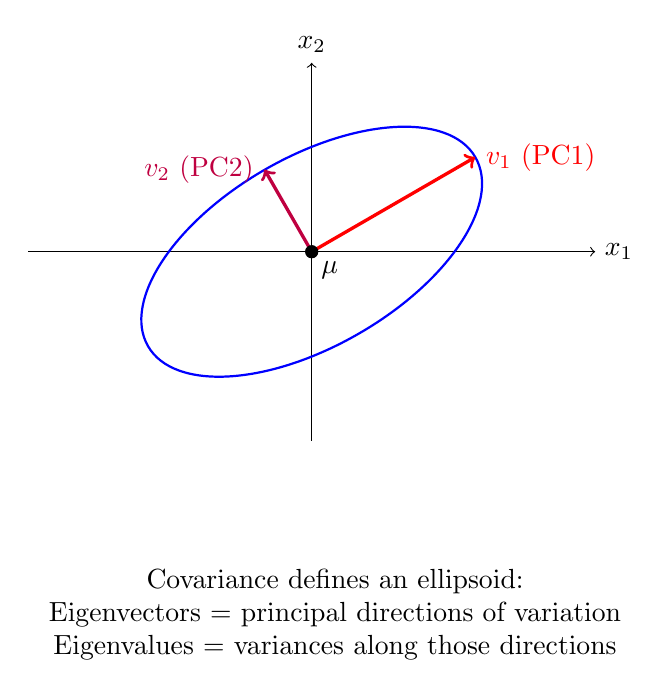
\begin{tikzpicture}[scale=1.2]
			% Axes
			\draw[->] (-3,0) -- (3,0) node[right] {$x_1$};
			\draw[->] (0,-2) -- (0,2) node[above] {$x_2$};
			
			% Covariance ellipse
			\draw[thick, blue, rotate=30] (0,0) ellipse (2cm and 1cm);
			
			% Principal axes (eigenvectors)
			\draw[->, very thick, red] (0,0) -- (1.73,1) node[right] {$\vect{v}_1$ (PC1)};
			\draw[->, very thick, purple] (0,0) -- (-0.5,0.87) node[left] {$\vect{v}_2$ (PC2)};
			
			% Mean
			\fill (0,0) circle (2pt) node[below right] {$\vect{\mu}$};
			
			\node[below=1.5cm, align=center] at (current bounding box.south) {
				Covariance defines an ellipsoid:\\
				Eigenvectors = principal directions of variation\\
				Eigenvalues = variances along those directions
			};
		\end{tikzpicture}
	\end{center}
\end{visualbox}

\section{Probability Distributions as Ontological Commitments}

\begin{seanbox}{2.3}
	\textbf{Common Distributions:}
	
	\begin{tabular}{ll}
		\textbf{Bernoulli:} & $P(X=1) = p$ \\
		\textbf{Binomial:} & $P(X=k) = \binom{n}{k} p^k (1-p)^{n-k}$ \\
		\textbf{Poisson:} & $P(X=k) = \frac{\lambda^k e^{-\lambda}}{k!}$ \\
		\textbf{Normal:} & $p(x) = \frac{1}{\sqrt{2\pi\sigma^2}} \exp\left(-\frac{(x-\mu)^2}{2\sigma^2}\right)$ \\
		\textbf{Exponential:} & $p(x) = \lambda e^{-\lambda x}$ \\
	\end{tabular}
\end{seanbox}

